\section{Sikkerhedsverifikation}
\begin{frame}{Sikkerhedsverifikation}{Omformulering af definition for barrierecertifikat}
\begin{block}{SOSTOOLS}
	\begin{itemize}
		\item Metodisk måde at søge barrierecertifikat for et system og dermed sikkerhedsvalidere det
		\item Kræver omformulering til sum of squares (SOS) problem
	\end{itemize}
\begin{equation*}
p(\mathbf{x})=\sum\limits_{j=1}^{m}f_j^2(\mathbf{x})=\mathbf{z}^T\mathbf{Q}\mathbf{z}\quad \in\Sigma[\mathbf{x}]
\end{equation*}
\end{block}
\begin{block}{Putinars Positivstellensatz}
	\begin{itemize}
		\item Gør det muligt at definere funktionens fortegn på de forskellige regioner
	\end{itemize}
\end{block}
\end{frame}

\begin{frame}{Barrierecertifikat-søgning med SOSTOOLS}{Sikkerhedsverifikation af lukketsløjfesystem}
%\begin{block}{Forståelse af værktøjet}
%		\begin{itemize}
%			\item Parametre til evaluering af resultat: feasibility ratio, residual norm, test om udtryk er SOS
%		\end{itemize}
%\end{block}
\begin{block}{Barrierecertifikat-søgning på slide use-case}
		\begin{itemize}
			\item Sikkerhedsverifikation af førsteordens system med lineær regulator for forskellige referencer
			\item Geometrisk forståelse af problemet
		\end{itemize}
\end{block}
\begin{figure}[h]
\begin{subfigure}[h]{.3\textwidth}
	\centering
	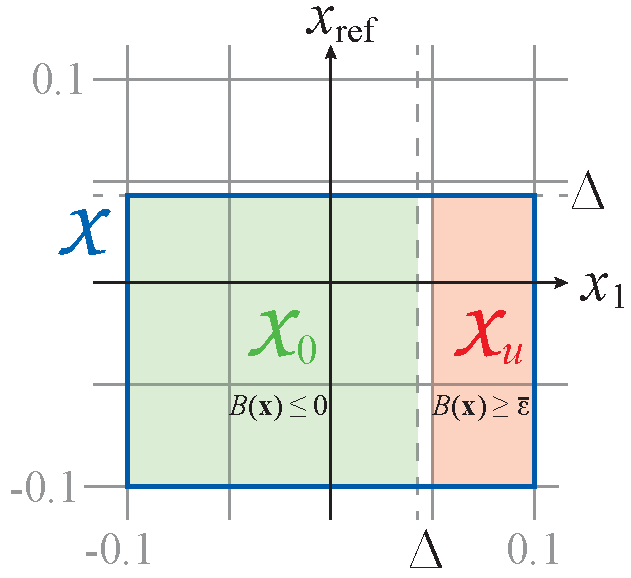
\includegraphics[width=\textwidth]{sos_Xregion.pdf}
\end{subfigure}
	\hspace{3mm}
\begin{subfigure}[h]{.3\textwidth}
	\centering
	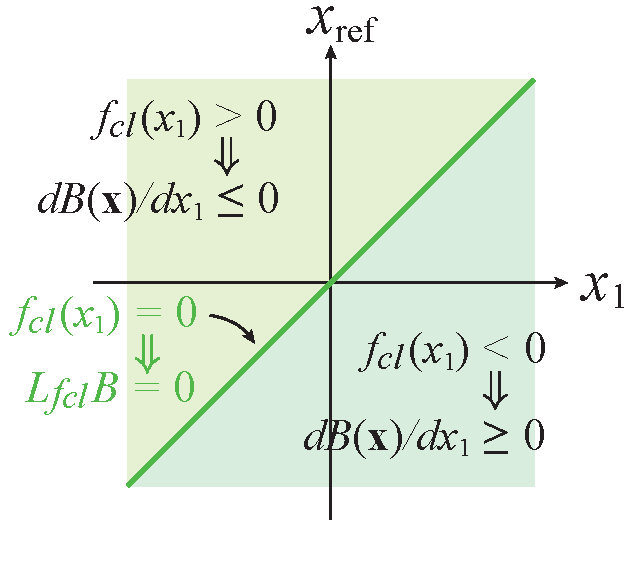
\includegraphics[width=\textwidth]{sos_Xregion_dBdx.pdf}
\end{subfigure}
	\hspace{3mm}
\begin{subfigure}[h]{.3\textwidth}
	\centering
	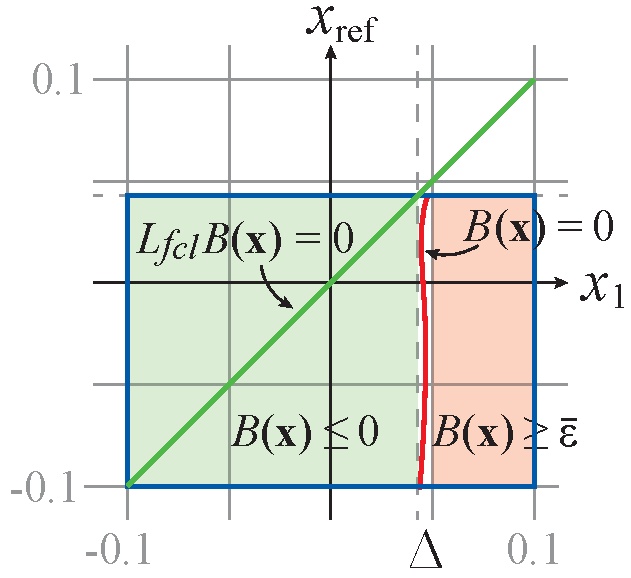
\includegraphics[width=\textwidth]{sos_Xregion_Bvalue.pdf}
\end{subfigure}
\end{figure}
\end{frame}

\begin{frame}{Barrierecertifikat-søgning med SOSTOOLS}{Sikkerhedsverifikation gennem fejl-tilstand}
	\begin{block}{Omformulering af problemet til fejl-tilstanden}
		\begin{itemize}
			\item Koordinatskifte og sammenhæng
			\item Forsimpling af problemet -- sikkerhedsverificering af både første- og andenordens model af slide-bevægelse
		\end{itemize}
	\end{block}
	\begin{figure}[h]
		\begin{subfigure}[h]{.3\textwidth}
			\centering
			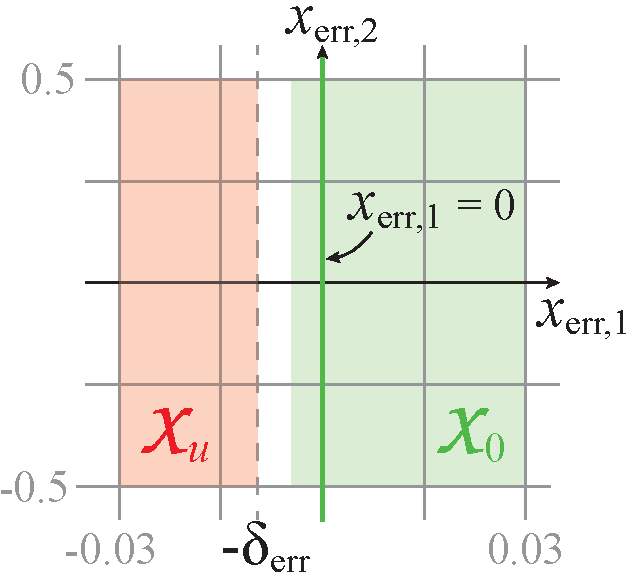
\includegraphics[width=\textwidth]{sos_error_2d_2ndorder.pdf}
		\end{subfigure}
		\hspace{3mm}
		\begin{subfigure}[h]{.3\textwidth}
			\centering
			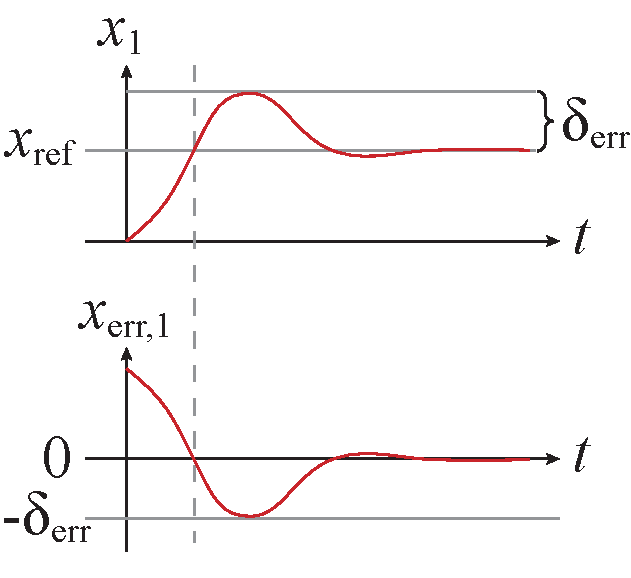
\includegraphics[width=\textwidth]{sos_delta_error_2ndorder.pdf}
		\end{subfigure}
		\hspace{3mm}
		\begin{subfigure}[h]{.3\textwidth}
			\centering
			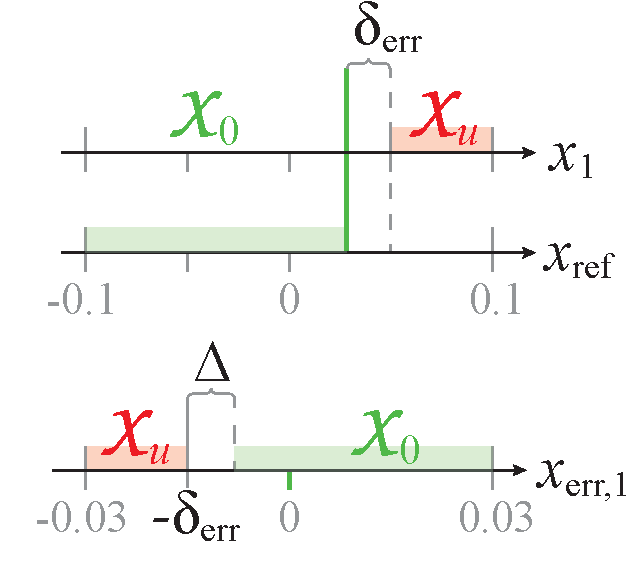
\includegraphics[width=\textwidth]{sos_errorref_1d_new_2ndorder.pdf}
		\end{subfigure}
	\end{figure}
\end{frame}

\begin{frame}{Evaluering af SOSTOOLS}{Sikkerhedsverifikation af lukketsløjfesystem}
	\begin{block}{Evaluering af løsning}
		\begin{itemize}
			\item Feasibility ratio, residual norm, test om ligninger er SOS
			\item Mange parametre at skrue på
			\item Længere proces at minimere numeriske fejl
		\end{itemize}
	\end{block}
	\begin{block}{Evaluering af værktøjet}
		\begin{itemize}
			\item Udviklet framework til søgning efter barrierecertifikater
			\item Fundet mange brugbare løsninger
			\item Systematisk afsøgning er en lang og iterativ proces
			\item Avanceret metode der kommer til sin ret for højere-ordens systemer
		\end{itemize}
	\end{block}
\end{frame}